\documentclass{article}
\paperwidth 10cm
\paperheight 5.8cm 
\usepackage[top=0.0cm,left=0cm,right=0cm,bottom=0cm]{geometry}
\usepackage{tikz}

\begin{document}
\begin{figure}[scale=0.6]
\centering
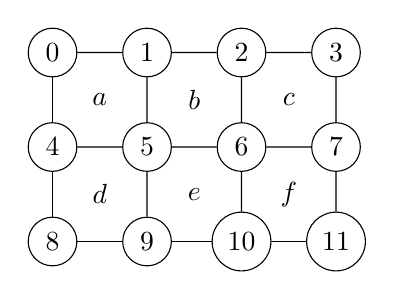
\begin{tikzpicture}[scale=0.6]
	\node (8) at (0,0) [shape=circle,draw] {$8$};
	\node (9) at (2,0) [shape=circle,draw] {$9$};
	\node (10) at (4,0) [shape=circle,draw] {$10$};
	\node (11) at (6,0) [shape=circle,draw] {$11$};
	\node (4) at (0,2) [shape=circle,draw] {$4$};
	\node (5) at (2,2) [shape=circle,draw] {$5$};
	\node (6) at (4,2) [shape=circle,draw] {$6$};
	\node (7) at (6,2) [shape=circle,draw] {$7$};
	\node (0) at (0,4) [shape=circle,draw] {$0$};
	\node (1) at (2,4) [shape=circle,draw] {$1$};
	\node (2) at (4,4) [shape=circle,draw] {$2$};
	\node (3) at (6,4) [shape=circle,draw] {$3$};
	\draw [-] (8) -- (9) -- (10) -- (11);
	\draw [-] (4) -- (5) -- (6) -- (7);
	\draw [-] (0) -- (1) -- (2) -- (3);
	\draw [-] (0) -- (4) -- (8);
	\draw [-] (1) -- (5) -- (9);
	\draw [-] (2) -- (6) -- (10);
	\draw [-] (3) -- (7) --(11);
	\node (a) at (1,3)  {$a$};
	\node (b) at (3,3)  {$b$};
	\node (c) at (5,3)  {$c$};
	\node (d) at (1,1)  {$d$};
	\node (e) at (3,1)  {$e$};
	\node (f) at (5,1)  {$f$};
\end{tikzpicture}
\caption{2 by 3 grid}
\end{figure}
\end{document}
